\id{МРНТИ 65.33.03}{https://doi.org/10.58805/kazutb.v.4.25-536}

\begin{articleheader}

	\sectionwithauthors{М.Т. Агедилова, А.М. Омаралиева, Ж.Т. Ботбаева, М.Б. Абилова}{НОҚАТ ҰНЫНЫҢ ЖӘНЕ ОДАН ДАЙЫНДАЛЫНҒАН ГЛЮТЕНСІЗ КОНДИТЕРЛІК
ӨНІМНІҢ МАЙ ҚЫШҚЫЛДЫ ҚҰРАМЫН ЗЕРТТЕУ}

{\bfseries \textsuperscript{1,3}М.Т. Агедилова\textsuperscript{\envelope },
\textsuperscript{1}А.М. Омаралиева, \textsuperscript{1,3}Ж.Т. Ботбаева,
\textsuperscript{2}М.Б. Абилова}
\end{articleheader}
\begin{affiliation}

\textsuperscript{1}«Қ.Қулажанов атындағы Қазақ технология және бизнес
университеті» АҚ, Астана, Қазақстан,

\textsuperscript{2}НАО «Казахский агротехнический университет им. С.
Сейфуллина», Астана, Қазақстан,

\textsuperscript{3}«ХБО» АҚ «Болашақ», Астана, Қазақстан


\raggedright{\bfseries \textsuperscript{\envelope }}Корреспондент-автор:
\href{mailto:agedilova-2011@mail.ru}{\nolinkurl{agedilova-2011@mail.ru}}

\end{affiliation}

Бұл зерттеудің мақсаты целиакиея ауруы бар адамдар үшін глютенсіз
тағамдардың (нан-тоқаш өнімдерінің) май қышқылдарының құрамын алғаш
аналитикалық тәсілмен зерттеу. Терапияның негізі глютенді тағамды күндік
рационнан толығымен алып тастау болып табылады. Бүгінгі күні дүкендерде
целиакиея ауруы бар науқастар үшін таңдауға болатын бірқатар глютенсіз
өнімдер бар, бірақ әліде жеткіліксіз немесе қымбат. Сондықтан, осындай
патологиясы бар адамдар үшін бидай ұнын қарақұмық, күрішпен, сұлы
жармасымен, жүгері жане ноқат дақылдар ұнымен алмастыру өте маңызды,
ғылыми тұрғыда бұл тақырыптың өзектілігін арттырады. Себебі, бұл дәнді-
дақылдар құрамы глютенсіз болуы және одан алынатын өнімнің тағамдық,
биологиялық құндылықтары жоғары болуы зерттеу жұмысын өзекті етеді.
Ноқат ұнының жоғары биологиялық құндылығы тек ақуыз мөлшерімен ғана
емес, сонымен қатар оның аминқышқылдық және жоғарғы май қышқылдарының
құрамдық мөлшерімен де бағаланады.

Бұл мақала зерттеуінде өңделмеген және өңделген ноқат ұнының, сондай-ақ
одан дайындалған өнімнің май қышқылдарының құрамы масс-спектрометриялық
газ хроматографиясының (ГХ/МС) көмегімен зерттелгені қарастырылған.

Осы зерттеуде ноқат ұнының глютенсіз кондитерлік өнімдерді өндіруге
жарамдылығын жақсарту бойынша біздің көзқарасымыз микротолқынды пеште
термиялық микротолқынды сәулеленумен (СВЧ) өңдеу арқылы ұнның тағамдық
құндылығын арттыруға негізделген. Зерттеу барысында ноқат ұны мен одан
жасалған өнімдердің құрамының сандық және сапалық өзгерістері зерттелді.
Зерттеу нәтижесі бойынша, ноқат ұнын термиялық өңдеу кезінде (мысалы,
профильтроли пісіру процесінде) жоғары майқышқылдық компоненттердің
құрамы өзгеретіні соңғы өнімнің тағамдық құндылығына әсер ететіні
қарастырылған. Дегенмен, ноқат ұнын пайдаланып жасалған жоғарғы
термиялық өңдеу процесінде оның өнімдерінің май-қышқылдық, ақуыздық және
тағамдық заттар құрамы қажетті мөлшерде қалады.

Алайда, ноқат ұны мен одан жасалған өнімдер биологиялық және тағамдық
құндылығы жоғары өнім болғандықтан арнайы диета ұстанатын тұтынушылар
мен денсаулығын қадағалайтын адамдарға, функционалды тамақтанушыларға
арналған тартымды тағам бола алады.

{\bfseries Түйін сөздер:} Ноқат, ноқат ұны, глютенсіз кондитерлік өнімдер,
май қышқылдарының құрамы, полиқанықпаған май қышқылдары, өңделмеген
ноқат ұны, өңделген ноқат ұны, \\масс-спектрометриялық газ хроматографиясы
\begin{articleheader}

{\bfseries ИССЛЕДОВАНИЕ ЖИРНОКИСЛОТНОГО СОСТАВА НУТОВОЙ МУКИ И
БЕЗГЛЮТЕНОВЫХ КОНДИТЕРСКИХ ИЗДЕЛИЙ}

{\bfseries \textsuperscript{1,3}М.Т. Агедилова\textsuperscript{\envelope },
\textsuperscript{1}А.М. Омаралиева, \textsuperscript{1,3}Ж.Т. Ботбаева,
\textsuperscript{2}М.Б. Абилова}
\end{articleheader}
\begin{affiliation}
\textsuperscript{1}«К. АО «Казахский университет технологии и бизнеса
имени Куладжанова», Астана. Казахстан,

\textsuperscript{2}НАО «Казахский агротехнический университет им. С.
Сейфуллина», Астана, Казахстан,

\textsuperscript{3}АО «ЦМП» «Болашак», Астана, Казахстан,

e-mail: agedilova-2011@mail.ru
\end{affiliation}

Целью данного исследования было изучение состава жирных кислот в
безглютеновых продуктах (хлебобулочных изделиях), для людей с целиакией
с использованием первого аналитического подхода. Основой терапии
является полное исключение глютена из ежедневного рациона. Сегодня в
магазинах имеется ряд безглютеновых продуктов, из которых пациенты с
целиакией могут выбирать, но они по-прежнему недостаточны или дороги.
Поэтому для людей с указанными патологиями очень важно то, что пшеничную
муку можно заменить гречневой, рисовой, овсяной, кукурузной и нутовой и
повышает актуальность темы с научной точки зрения. Потому что, это
связано с тем, что состав этих круп не содержит глютена и высокая
пищевая, биологическая ценность получаемых из него продуктов делают
исследовательскую работу актуальной. Высокая биологическая ценность
нутовой муки оценивается не только содержанием в ней белка, но и
составом аминокислот и жирных кислот.

В данной статье рассмотрено, что состав жирных кислот необработанной и
переработанной нутовой муки, а также продуктов, приготовленных из нее,
изучен методом масс-спектрометрической газовой хроматографии (ГХ/МС). В
данном исследовании наш подход к повышению пригодности нутовой муки для
производства безглютеновых кондитерских изделий основан на повышении
пищевой ценности муки путем обработки микроволновым тепловым излучением
(ЖЖӨ/СВЧ). В ходе исследований изучены количественные и качественные
изменения в составе нутовой муки и изделий из нее. По результатам
исследований считается, что при термической обработке нутовой муки
(например, в процессе приготовления профильтроли) изменяется состав
высокожирных кислотных компонентов, что влияет на пищевую ценность
конечного продукта. Однако в процессе с использованием термической
обработки жирные кислоты, белки и питательные вещества нутовой муки и ее
продуктов сохраняются в необходимом количестве.

Однако нутовая мука и продукты из нее являются продуктом высокой
биологической и пищевой ценности, что делает ее привлекательным
продуктом питания для специалистов по функциональному питанию, для
потребителей, соблюдающих специальную диету, и для людей, заботящихся о
своем здоровье.

{\bfseries Ключевые слова:} Нут, нутовая мука, безглютеновые кондитерские изделия,
жирнокислотный состав, полиненасыщенные жирные кислоты, необработанная
нутовая мука, обработанная нутовая мука, масс-спектрометрической газовой
хроматографии.
\begin{articleheader}

{\bfseries STUDY OF FATTY ACID COMPOSITION OF CHICKEAT FLOUR AND
GLUTEN-FREE CONFECTIONERY PRODUCTS}

{\bfseries \textsuperscript{1,3}M.T. Agedilova\textsuperscript{\envelope },
\textsuperscript{1}A.M. Omaralieva, \textsuperscript{1,3}Zh.T. Botbaeva,
\textsuperscript{2}M.B. Abilova}
\end{articleheader}
\begin{affiliation}
{\bfseries \textsuperscript{1}} «K. JSC "Kazakh University of Technology
and Business named after Kulajanov», Astana. Kazakhstan,

{\bfseries \textsuperscript{2}} NAO «Kazakh Agrotechnical University named after. S. Seifullin»,
Astana, Kazakhstan,

{\bfseries \textsuperscript{3}}  JSC «CMP» «Bolashak», Astana, Kazakhstan,

e-mail: agedilova-2011@mail.ru
\end{affiliation}

The aim of this study was to examine the fatty acid composition of
gluten-free foods for people with celiac disease using a first
analytical approach. The basis of therapy is the complete exclusion of
gluten from the daily diet. Today there are a number of gluten-free
products available in stores from which celiac disease patients can
choose, but these are still insufficient or expensive. Therefore, for
people with these pathologies, it is very important that wheat flour can
be replaced with buckwheat, rice, oatmeal, corn and chickpeas and
increases the relevance of the topic from a scientific point of view.
Because this is due to the fact that the composition of these cereals
does not contain gluten and the high nutritional and biological value of
the products obtained from it make the research work relevant The high
biological value of chickpea flour is assessed not only by its protein
content, but also by the composition of amino acids and fatty acids.

This article discusses that the fatty acid composition of raw and
processed chickpea flour, as well as products prepared from it, was
studied by gas chromatography mass spectrometry. In this study, our
approach to improve the suitability of chickpea flour for gluten-free
confectionery production is based on enhancing the nutritional value of
the flour through microwave thermal treatment. During the research,
quantitative and qualitative changes in the composition of chickpea
flour and products made from it were studied. According to research
results, it is believed that heat treatment of chickpea flour changes
the composition of high-fatty acid components, which affects the
nutritional value of the final product. However, in the process using
heat treatment, the fatty acids, proteins and nutrients of chickpea
flour and its products are retained in required quantities. However,
chickpea flour and products made from it are a product of high
biological and nutritional value, which makes it an attractive food
product for functional nutritionists, for consumers on special diets and
for people concerned about their health.

However, chickpea flour and products made from it are a product of high
biological and nutritional value, which makes it an attractive food
product for functional nutritionists, for consumers on special diets and
for people concerned about their health.

{\bfseries Keywords:} Chickpeas, chickpea flour, gluten-free confectionery,
fatty acid composition, \\polyunsaturated fatty acids, unprocessed
chickpea flour, processed chickpea flour, gas chromatography mass
spectrometry.

\begin{multicols}{2}

{\bfseries Кіріспе.} Қазақстан халқының салауатты тамақтануының өзекті
мәселелерінің бірі жергілікті отандық шикізатты өңдей отырып,
ақуыздармен, алмастырылмайтын аминқышқылдарымен, қанықпаған май
қышқылдарымен, минералдармен, витаминдермен және талшықтармен байытылған
нан және нан-кондитерлік өнімдерін өндіру маңызды бағыттардың бірі болып
табылады. Бұл тұрғыда мақалада қарастырылып отырған шикізат көзі ноқат
маңызды болып табылады. Ноқаттың тағамдық құндылығы оның құрамындағы
ақуыздың жоғары болуына байланысты. Ноқаттың құрамында шамамен 20-25\%
протеин бар, бұл оларды өсімдік негізіндегі ақуыздың тамаша көзі етеді,
әсіресе вегетарианшылар мен глютенге төзбейтін адамдар үшін өте қажет.
Ноқат құрамы тіпті маңызды аминқышқылы, яғни тамақтануды баланста
ұстауға мүмкіндік беретін лизинге де бай. Моноқанықпаған май қышқылдары
(МНЖК) құрамдас бөліктер (57\%), одан кейін қаныққан май қышқылдары
(НЖК) (30\%) және полиқанықпаған май қышқылдары (13\%) бар {[}1{]}.

Ноқат өнімдерінің құрамы жүрек-қан тамырлары дұрыс жұмысына жауап
беретін пайдалы май қышқылдарына да бай. Ноқат - жалпы денсаулыққа аса
қажет темір, магний, фосфор сияқты пайдалы заттар және В дәрумендерінің
жақсы көзі. Ноқаттағы диеталық талшықтың жоғары мөлшері ас қорыту
жүйесін қалыпқа келтіруге және метаболизмді жақсартуға көмектеседі
{[}2{]}. Жалпы тағамдық мақсатта қолданылатын ноқат ГОСТ 8758-76
қарастырылады, сонымен қатар медициналық-биологиялық талаптармен және
тамақ шикізаты мен азық-түлік өнімдерінің сапасының санитарлық нормалары
СанЕж/еН 1.3.2.1078-01 сәйкес жүргізіледі {[}3, 4{]}.

Осы зерттеуде ноқат ұнының глютенсіз кондитерлік өнімдерді өндіруге
жарамдылығын жақсарту бойынша микротолқынды пеште (СВЧ) термиялық өңдеу
арқылы ұнды өңдеуге негізделген {[}5{]}. Жоғары температура қамырдың
икемділігі мен құрылымын жақсартатын крахмал желатинизациясын (шикізат
құрамы бойынша) және ақуыздың денатурациясын жақсартады. Қамырдың дұрыс
консистенциясына жету үшін оңтайлы ылғалдылық деңгейі қажет. Шамадан тыс
немесе жеткіліксіз ылғалдылық жағымсыз текстуралық қасиеттерге және
дайын өнімнің сапасыздығына әкелуі мүмкін. Термиялық және ылғалды
өңдеуде уақыт та өте маңызды. Тым қысқа уақыт қажетті нәтиже бермеуі
мүмкін, ал шамадан тыс өңдеу маңызды тағамдық компонентердің жоғалуына
және органолептикалық қасиеттердің нашарлауына әкелуі мүмкін. Сондықтан
бұл зерттеу барысында температура (t°C), ылғалдылық (\%) және уақыт (Ʈ,
минут) сияқты параметрлердің ноқат ұнының қамыры мен одан жасалатын
кондитерлік өнімдерді дайындап өңдеу жағдайларына байланысты
сипаттамалық кқрсеткіштеріндегі айырмашылықтардың болуын анықтап,
дайындатын жаңа глютенсіз кондитерлік өнімнің дайындалу процесінің
оптималды режиміндерін зерттеуге арналды. Осылайша, бұл шарттарды
оңтайландыру қажетті қасиеттері бар сапалы глютенсіз кондитерлік
өнімдерді дайындаудың негізгі кілті болып табылады.

Зерттеуде микротолқынды термиялық өңдеу арқылы ноқат ұнының глютенсіз
кондитерлік өнімдерді өндіруге жарамдылығын арттыру өте перспективалы
болып көрінеді. Бұл әдіс ұнның физикалық қасиеттерін өзгертуге, оның
құрылымы мен функционалдығын жақсартуға көмектеседі. Микротолқынды пеште
(СВЧ) өңдеу крахмалдың желатинденуіне, қамырдың тұтқырлығын жақсартуға
және серпімділікті арттыруға көмектеседі. Бұл дәстүрлі ингредиенттер
қажетті сипаттамаларды бере алмайтын глютенсіз өнімдер үшін өте маңызды.
Сонымен қатар, бұл тәсіл қоректік заттардың биожетімділігін арттырып,
микробиологиялық қауіпсіздікті жақсарта алады. Бұл бағыттағы
зерттеулердегі процестер мен тұжырымдарды оңтайландыруға көмектеседі,
яғни өз кезегінде жақсырақ және дәмді глютенсіз өнімдерді жасауға
әкеледі {[}6, 7{]}.

Микротолқынды өңдеу шын мәнінде дәнді дақылдар мен жалған дәнді
дақылдарды термиялық және ылғалдылықпен өңдеудің жылдам және үнемді
әдісі болып табылады. Бұл әдісте материалды біркелкі қыздыруға мүмкіндік
береді, бұл оның текстуралық және функционалдық қасиеттерін жақсартуға
көмектеседі. Өңдеуде микротолқынды пешті пайдаланғанда температураның
тез арада жоғарылауы байқалады, бұл крахмалдың қажетті желатинизациясына
және ақуыздардың денатурациясына әкелетіні түсінікті. Бұл әсіресе
глютенсіз өнімдер үшін маңызды, себебі өз кезегінде, ұнның байланыстыру
қасиеттерін жақсартады. Сонымен қатар, микротолқынды пеште өңдеу бу
немесе жылу өңдеу сияқты дәстүрлі әдістермен салыстырғанда уақыт пен
қуат шығындарын азайтуға көмектеседі. Бұл ұн мен дайын өнімнің сапасын
тиімді жақсартуға мүмкіндік беретін өнеркәсіптік өндіріс үшін маңызды
тәсілді {[}8, 9, 10{]}.

Бұл зерттеулер ноқат ұнынан жасалған қамыр мен оның кондитерлік
өнімдерінің температура, ылғалдылық және уақытқа тәуелділігі сияқты
өңдеу жағдайларына байланысты параметрлік сипаттамалары айтарлықтай
өзгеруі мүмкін екенін көрсетеді. Осылайша, осы шарттарды оңтайландыру
қажетті қасиеттері бар сапалы глютенсіз кондитерлік өнімдерді жасаудың
және осы бағытты дамытудың кілті болып табылады.

Глютенсіз өнімдер бағыты бойынша жарма және бұршақ дақылдары сияқты
әртүрлі шикізат түрлерін қолдануға деген қызығушылықтың артуына
қарамастан, олардың ұнынан алынган қамырдың реологиялық және термиялық
қасиеттеріне әсер етуші оптималды факторлар сипаттары әлі де аз
зерттелгендігі тақырыптың өзектілігін көрсетеді. Бұл қасиеттерді түсіну
сапалы композициялық ұн қоспаларын жасау үшін маңызды, өйткені ұнның
әртүрлі түрлері қамырдың құрылымына, серпімділігіне және тұрақтылығына
айтарлықтай әсер етуі мүмкін.

Оңтайлы ұн комбинацияларын және олардың соңғы өнімнің физикалық
сипаттамаларына әсерін анықтау үшін қосымша зерттеулер қажет. Бұл бізге
жақсартылған қасиеттері бар глютенсіз өнімдерді өндіру үшін тиімдірек
рецептуралар мен технологияларды әзірлеуге мүмкіндік береді.

Ноқат ұнын өңдеу оны қолданып нан және кондитерлік өнімдерін жасау
Қазақстан халқының тамақтану жолының дұрыс және сапасын арттырудың
маңызды бағыты болып та табылады. Перспективалы шикізатты пайдалану
диеталық кондитерлік ассортиментті байытып қана қоймай, сонымен қатар
халықтың денсаулығы мен әл-ауқатын жақсартуға көмектеседі.

Биологиялық құндылығы жағынан ноқат жасымық пен бұршақтан жоғары, соядан
кейін екінші орында, сондықтан ноқат қосылған өнімдерде ақуыздың мөлшері
артып қана қоймай, оның сапасы да жақсарады. Ноқат белоктарында лизин,
метионин, треонин және триптофанның жоғары мөлшері бар.

Ноқат тұқымында фосфор -- 290 мг/100 г, калий және магний -- 126 мг/100
г айтарлықтай мөлшерде. Бұл кальций мен фосфордың 1:1,5 қатынасымен
ерекшеленетін бірнеше бұршақ тұқымдас дақылдардың бірі.

Ноқатта селеннің болуы өте құнды -- 0,5 мг/100 г (өнімге шаққанда)
құрайды, темір -- 18,7, мырыш -- 2,87 мг/100 г. Ноқат лецитиннің,
рибофлавиннің (B2), тиаминнің (B1), никотин және пантотен қышқылдарының,
холиннің және басқа дәрумендердің жақсы көзі болып табылады.

Диетада ноқат өнімдерін пайдалану әлсіреген өкпе белсенділігін нығайтуға
көмектеседі және суық тию мен бронх ауруларын жояды. Ноқаттағы магнийдің
болуы бас айналуды жоюға көмектеседі, қан қысымын қалыпқа келтіреді,
жүрек пен қан тамырларының бұлшықеттерін қорғайды.

Ноқат құрамындағы кальций тістерді, сүйектерді және жүрек бұлшықеттерін
баланста ұстау үшін қажет. Селен ағзадағы гемопоэз процесін
тұрақтандыру, ондағы қатерлі түзілімдерді тежеу және остеопороздың алдын
алу үшін қажет {[}11{]}.

Осы тұрғыдан алғанда бұршақ тұқымдас дақылдары диеталық және
профилактикалық бағыттағы аса зор перспективалы шикізат болып табылады.
Сондай дақылдардың бірі -- ноқат. Биологиялық құндылығы жағынан ноқат
жасымық және бұршақ сияқты бұршақ тұқымдас дақылдардан жоғары, соядан
кейін екінші орында. Сондықтан ноқат қосылған өнімдерде ақуыздың мөлшері
артып қана қоймай, оның сапасы да жақсарады. Ноқат ұнының биологиялық
құндылығы тек ақуыз мөлшерімен ғана емес, оның салмағы мен құрамдас
компоненттерімен, сондай-ақ май қышқылды қосылыстарымен де анықтайды.

Әдебиеттік шолу бойынша, май қышқылдарының жалпы мөлшері 100 г өнімінде
-7,7\% (4,32 г) құрайды, оның 13\%-ы қаныққан май қышқылдары, 20\% -ы
бір қос байланысты моноқанықпаған қышқылдан және 67\% -ы полиқанықпаған
май қышқылдары болып келеді. Полиқанықпаған май қышқылдары сарысудағы
холестерин деңгейін белсенді түрде төмендетеді; моноқанықпаған - қан
сарысуындағы холестеринге тәуелсіз әсер етпейді. Бұл шиізатты немесе
одан алынған өнімдерді өңдегенде, оның тағамдық май қышқылдарының
мөлшерін арттыруда негізгі рөл атқаратын қаныққан май қышқылдары
қатарына жатады. Полиқанықпаған май қышқылдарының болуы қан тамырларының
қабырғаларында ауыр холестерин концентрациясын болдырмайтын
простагландиндердің түзілуіне жағдай жасайды {[}12{]}.. Полиқанықпаған
май қышқылдары маңызды қоректік заттар болып табылады. Олардың айқын
антиатерогендік әсері бар {[}13{]}. Эксперименттік зерттеулер
көрсеткендей, адам рационына полиқанықпаған май қышқылдарын жүйелі түрде
қосымша енгізу жүректің ишемиялық ауруы, дисциркуляторлы энцефалопатия
және аяқтың төменгі жағындағы артериялардың окклюзиялық аурулары сияқты,
атеросклероздан туындаған аурулардың дамуы мен асқыну қаупін айтарлықтай
алдын алып төмендетуге мүмкін жасайды {[}14{]}.

Осыған байланысты зерттеудің мақсаты биобелсенді ноқат ұнының негізінде
биологиялық құндылығы жоғары глютенсіз кондитерлік өнімдер дайындауда
физикалық параметрлердің майқышқылдық құрамына әсерін зерттеу. Бұл
зерттеуде мақсаты микротолқынды пеште (СВЧ) ноқат ұнының өңделмеген,
яғни өңдеуге дейін және одан кейінгі алынған ұнының майлы қышқылдық
құрамын зерттеу және өңделген ұн негізінде дайындалған жаңа кондитерлік
өнім (профильтроли) және жартылай фабрикаттармен салыстыру. Қолданылатын
сынақ объектілері ноқат ұны және глютенсіз кондитерлік өнімдер болып
табылады. Ноқат ұнына негізделген глютенсіз кондитерлік өнімдерді
әзірлеу кезінде микротолқынды пеште (СВЧ) алдын - ала өңдеу ұсынылады.

{\bfseries Материалдар мен әдістер.} Зерттеуде бакылау үлгісі ретінде өңделген ноқат ұны және одан
дайындалған жаңа глютенсіз кондитерлік өнім (профильтроли) және
салыстырмалы бақылау үлгісі --өңделмеген ноқат ұны алынды.

Үлгілерді масс-спектрометриялық газ хроматографиясының (ГХ/МС) әдісімен
эсперименттік зерттеп талдау Е.Бөкетов атындығы Қарағанды
университетінің «Физика-химиялық зерттеу әдістері» инженерлік бейіндегі
аккредиттелген зертхана орталығында жасалды.

Бақылау үлгісі ретінде алынған өңделмеген ноқат ұнымен өңделген ноқат
ұны және глютенсіз өнімнің (профильтроли) май-қышқылдық құрамы
масс-спектрометриялық газ хроматографиясының (ГХ/МС) әдісімен анықталды.
Ноқат ұнының компоненттік құрамын анықтау үшін экстракция және
хроматографиялық әдістер көмегімен талдау жүргізілді.

Экстракция процесі: Алдымен өңделмеген ноқат ұнының құрамдас
компоненттік құрамын анықтау үшін экстракциялау жүргізілді. Экстракция
10 мл хлороформ 8 г үлгі(лермен) араластырылды, қоспаны бір минут
шайқап, бөлгіш сүзгіште сүзеді және 5 мл хлороформмен қайта шаймалап
шаяды. Әр үлгі осы әдіспен үш рет қайталанады. Экстракциялау процесінде
алынған біріктірілген сығынды күйдірілген MgSO4-пен кептірілді және 1,5
мл-ге дейін буланды. Алынған үлгілерге масс-спектрометриялық газ
хроматографиясының (ГХ/МС) Agilent 7890A газ хроматографы пайдаланылып
талдау жүргізілді. Бұл әдіс май қышқылдарының сандық және сапалық
құрамын анықтауда жоғары сезімталдық пен дәлдікті қамтамасыз етеді.

Үлгілер газ хроматографиясының Agilent 5975°C массалық селективті
детекторы бар аппарат көмегімен талданып зерттелді.

Талдау келесі шарттарда жүргізілді: баған түрі -- Rxi-5ms, баған
ұзындығы -- 30 м; баған диаметрі -- 0,25 мм; колонна адсорбентінің
қалыңдығы -- 0,25 мкм, буландырғыш температурасы -- 250 °C; термостат
температурасы -- 60-300 °C; тасымалдаушы газ -- гелий; тасымалдаушы газ
шығыны --1 мл/мин; бағандағы газ қысымы -- 54,51 кПа; үлгі көлемі --0,2
мкл.

Нәтижелер GS-MSD Data Analysis бағдарламасы арқылы автоматты түрде
өңделді. Эксперимент нәтижелерінің масс-спектрограммалары үлкейтілген
түрде 1-3 суретте мақалада келтірілген.

{\bfseries Нәтижелер мен талқылаулар.} Ноқат ұны - өңделмеген (салыстырмалы бақылау нұсқасы), өңделген ұн --
негізгі шикізат және одан дайындалған кондитерлік өнімнің
(профильтролидің) масс спектроскопияда детекторлық бөлініп алынған
липофильді кешеннің құрамын және құрамдас май қышқылдарының пайызын
зерттеу нәтижелерінің талдауы 1-3-суреттерде келтірілген.

Талдау бойынша, өңделмеген ноқат ұнында (салыстырмалы бақылау үлгісі) 22
қосылыс бары анықталған. Ал зерттеу барысында термиялық өңдеуден өткен
ноқат ұнында 26 қосылыс спектрометрияда байқалды. Бұл яғни эсперименттік
зерттеудің ерекшелігі, ноқат ұнын термиялық өңдеу кезінде улы заттардың
сандық құрамының азайып, тағамдық құндылығы жоғарлайтыны және жаңа
алынатын өнімнің пайдалы қосылыстарының пайыздық мөлшерінің артатыны
және тағам шикізатында болатын зиянды компоненттердің модификациялануы
байқалатыны зерттеу барысында дәлелденді.

Мысалы, барлық азық-түлік өнімдерінде маңызды құрамдас болып саналатын
линол, линолен, олеин және пальмитин қышқылдарының, стеарин қышқылының
метил эфирінің, фталь қышқылының және дәрумендер қатарының, яғни
dl-альфа- және гамма-токоферолдардың ең жоғары мөлшерібар екені
анықталды. Зерттеудің алғашқы кезеңінде өңделмеген ноқат ұны
Масс-спектрометриялық газ хроматографиясының (ГХ/МС) өңделмеген ноқат
ұнының (NE\_OBR\_NUT\_MUKA) хроматограммасы 1-суретте келтірілген.


Зерттеу нәтижесі бойынша хроматограмма көрінісі май қышқылының құрамы
бойынша өңделмеген ноқат ұнының (NE\_OBR\_NUT\_MUKA) үлгісін талдау
кезінде зерттеу нәтижелері 30 минут ішінде хроматограмма бойынша көріну
уақыты 35,821 минуттан - 61,511 минут аралығында 22 қосылыс анықталғанын
көрсетті.

Хроматограммалар бойынша өңделмеген ұн шикізатының негізгі құрамдас
бөліктері: токоферол -- 7,02\%, Е витамині -- 3,11\%, пальмитин қышқылы
-- 2,16\%, стеарин қышқылының метил эфирі -4,35\%, линол қышқылы --
3,57\%, адипин қышқылыгың үлесі 9,2\% пайызды құрайтынын және o-фталь
қышқылы тек 0,62\% және басқа қосылыстар бар екенін көруге болады.
\end{multicols}

\begin{figure}[H]
	\centering
	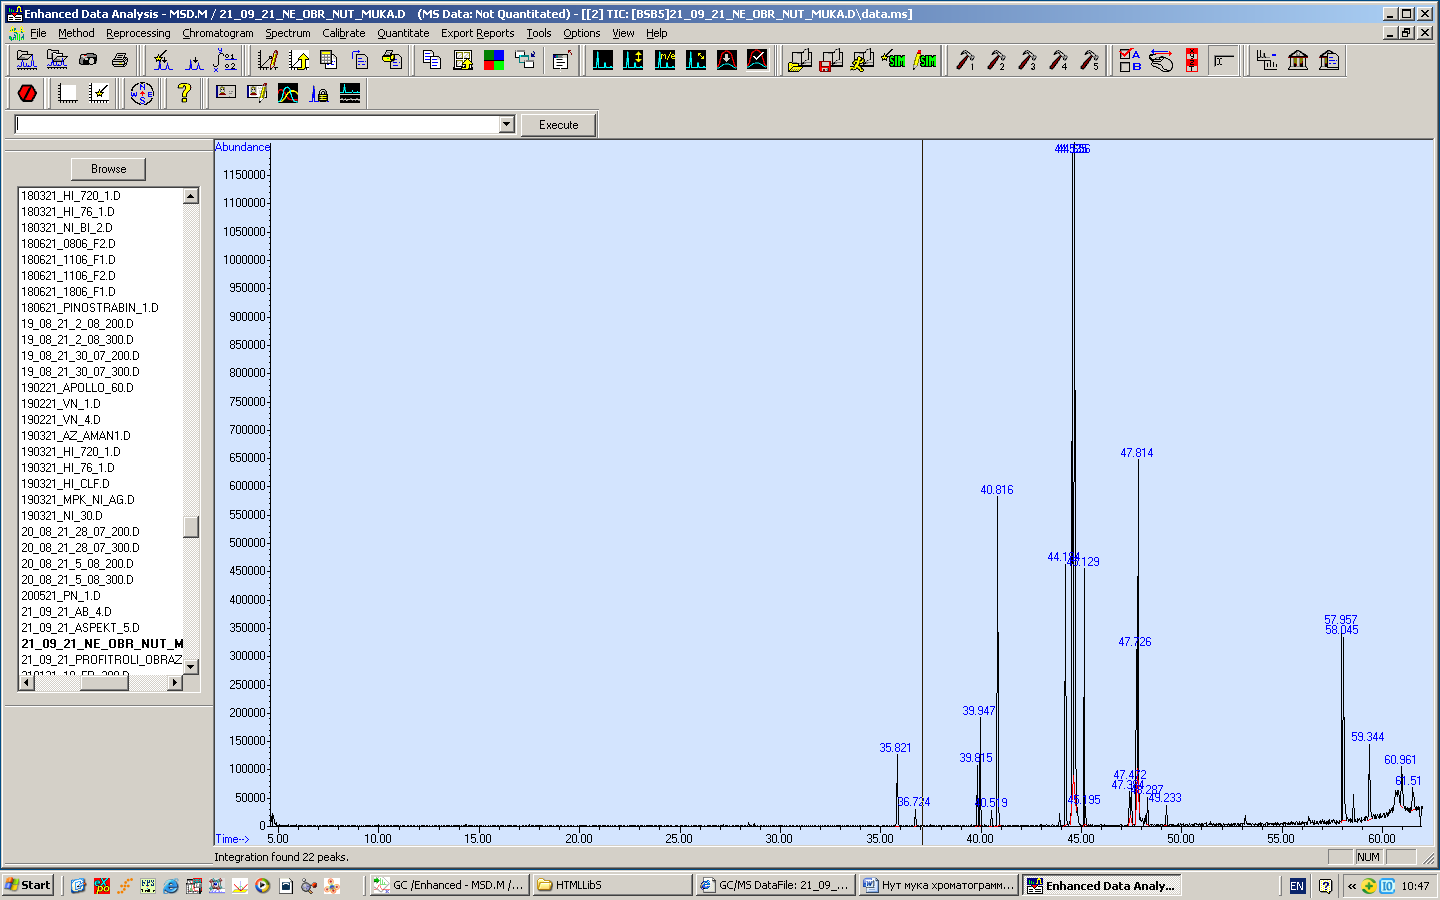
\includegraphics[width=0.8\textwidth]{media/pish/image13}
	\caption*{1-сурет. Өңделмеген ноқат ұнының хроматограммасы
	(NE\_OBR\_NUT\_MUKA)}
\end{figure}


\begin{multicols}{2}

Өңделмеген ұнда канцерогенді қосылыстардың пайыз мөлшері жоғары және
хроматоргаммада байқалу уақыты 40,816 минуттан-44,656 минтуттар
арадығында, яғни 11,00-20,96 \% аралығында байқалады. Табиғи ноқаттың
құрамында ұнды өңдегеннен кейін және өнімдерді дайындау кезінде
анықталған каприл амиді термиялық (СВЧ) өңдеудің барысында
модификациялануының нәтижесінде тиісті көріну аймағы уақытында 10--12\%
үлесте стеарин қышқылының метил эфирі сияқты құнды тағамдық компонентке
дейін айналатыны байқалды. Сондай-ақ өңделмеген ұнның құрамындағы
5-Хлоро-3-{[}2-этрагидропиранилметил{]}-4(3Н)-хиназолон (20,00\%),
пиперидин N-этил-4-{[}1-аминоэтил{]} сияқты қосылыстар да өңделген ноқат
ұнындағы мөлшері (хроматограммада сурет -1 тиісті шығу уақытында) -
2,78\%-ға дейін төмендегені, ал жаңа дайындалған өнімде (профильтролиде)
ол небәрі 0,59\%-ды құрады.

2-бензотиазолсульфенамидтің өңделген ноқат ұнында 20,96\% мөлшері
өңделген түрінде- 3,05\%-ға дейін төмендейді, ал жаңадан жасалған
кондитерлік өнімде (профильтролиде) ол тек 0,76\% құрады.

Бұл нәтежелер бойынша келесі тұжырым жасайға болады: термиялық өңдеу
(ЖЖӨ) барысында табиғи заттар құрамындағы құрамдас кейбір улы,
концереогенді заттар модификациялануы барысында тағамдық құндылығы
жоғары қосылыстарға алмасатынындығын байқауға болады, бұл әдістің арзан
және тиімділігін көрсетеді.

Сонымен қатар, өңделмеген ұнның құрамында Е 355 дозалық тағамдық қоспасы
(адипин қышқылы) 9,20\% мөлшерде болды. Бұл қышқыл антиоксидант қызметін
атқарады және тамақ өнеркәсібінде қышқылдандырғыш және тағамды
мерзімінен бұрын бұзылудан және қышқылданудан қорғауда консервант
ретінде қолданылады. Тамақ өнеркәсібінде сонымен қатар, E355 тағамдық
қоспасы бар тағамдар мен сусындарға (негізінен алкогольсіз) қышқыл дәм
беруге арналған, бірақ ол 2-қауіптілік сыныбы қатарына кіреді. Жалпы, ол
адамға зиянсыз деп саналады. Бірақ негізінен дозасын және пайдалану
ережелерін сақтамауға байланысты денсаулыққа қауіп төндіреді. Адипат
ионына негізделген тәулігіне дене салмағының әр кг-на 5 мг-нан аспайтын
мөлшерін тұтынуға рұқсат етіледі. Судағы ең жоғары рұқсат етілген
концентрациясы 1 литрге 2 мг құрайды. Ал жаңа дайын өнімнің (3-сурет)
бойынша хроматограммасында бұл көріну аймағы уақытында қоспаның
модификацияланғандығы байқалып, тағамдық қышқыл - линол қышқылы басқанын
және оның 9,65\% мөлшер шамасында байқалғаны анықталды. Линол қышқылы
-C=C- қос байланысының болуына байланысты полиқанықпаған май қышқылының
мысалы болып табылады. Бұл соя, жүгері сияқты өсімдік майларында
кездесетін негізгі май қышқылы. Ол маргарин, асханалық майлар, сонымен
қатар сабын, эмульгаторлар және тез кептіргіш майлар алу үшін де
қолданылады. Линол қышқылы адам мен жануарлар ағзасына қажетті
алмастырылмайтын май қышқылдарының екі класының біріне жатады. Егер адам
осы маңызды май қышқылдарын жеткілікті мөлшерде тұтынбаса, денсаулығына
байланысты бірқатар қиындықтар туындауы мүмкін. Линолеаттың (қышқылдық
тұз түрі) жеткіліксіз мөлшері бар және эксперимент бойынша анықталған,
диеталар терінің қалыпты зақымдалуын, шаштың түсуін және терінің қалпына
келуін бұзуды тудырады.

Сонымен қатар мақалада зерттеу бойынша 2-суретте көрсетілгендей өңделген
ноқат ұнының май қышқылдық құрамының талдауы келтірілген. Өңделген ноқат
ұнының компоненттік құрамының үлгісіне (OBR\_NUT\_MUKA) зерттеу
барысында нәтиже келесі көріністі бере отырып (2-суретте) - 26
қосындының бар екені айқындалды.
\end{multicols}


\begin{figure}[H]
	\centering
	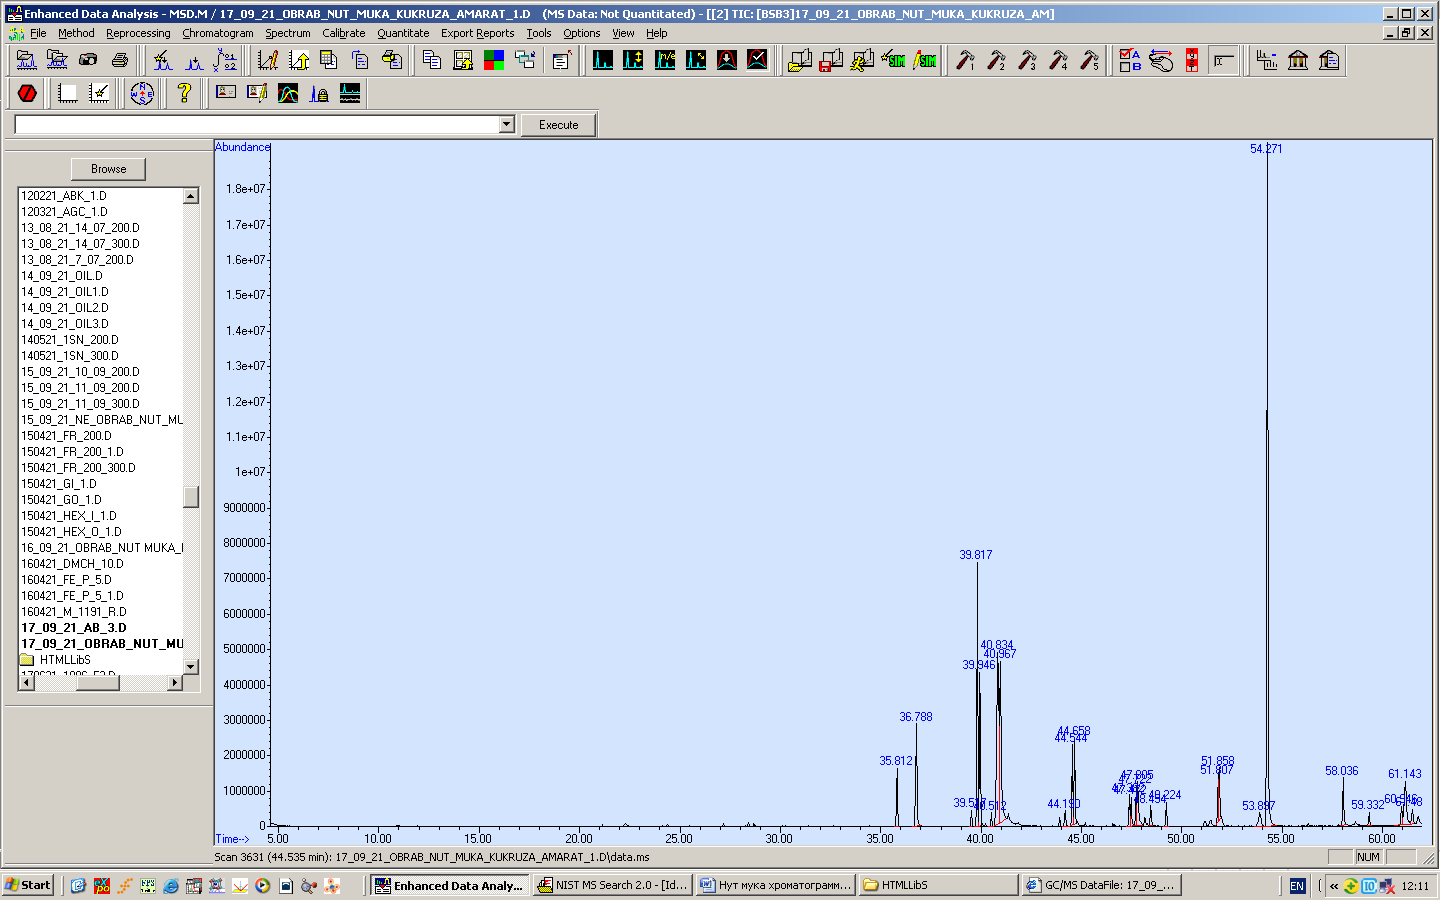
\includegraphics[width=0.8\textwidth]{media/pish/image14}
	\caption*{2-сурет. Өңделген ноқат ұнының хроматограммасы (OBR\_NUT\_MUKA)}
\end{figure}


\begin{multicols}{2}

Зерттеудің талдау нәтижесі бойынша, өңделмеген ноқат ұнымен
салыстырғанда бұл нысанда компоненттердің саны 4 қосылысқа артқаны
анықталды, яғни микротолқындық пеште термиялық СВЧ әдіспен өңдеу
заттардың модификациясына әкелетіні анықталды.

Микротолқынды пеште өңдеуден кейін өңделген ноқат ұнында олеин қышқылы
10,36\% құрады, ол хроматограммада өңделмеген ұн құрамында жоқ және
тағамдық линол қышқылы жоғары мөлшерде (28,10\%) алдыңғы зерттеу бойынша
өңделмеген ноқат ұнының құрамымен (3,57\%) салыстырғанда 7,9 есе артық
екені анықталды, бұл зерттеудің көрсеткіштері жоғарыда айтылып өткен
критерийлердің дәлелі болып табылады.

Зерттеу бойынша тағамдық қышқылдардың құрамында пальмитин қышқылының
жалпы мөлшері 7,04\%-ға екі есе өсті (өңделмегенде ұнда ол 2,16\%-ды
құрады), стеарин қышқылының метил эфирі жалпы май қышқылдарының үлесінің
4,35\%-дан 30,79\%-ға дейін ауытқитыныны байқалды. Бұл аналитикалық
көрсеткіштер стеарин қышқылының метил эфирінің жоғарылауы, пальмитин
қышқылының өңделген үлгіге қарағанда екі есе көп болуы, үлгіні
микротолқынды пешпен өңдеу кезінде тағамдық құндылығының жоғарылағандығы
байқалады.

Өңделген ноқат ұнындағы табиғи Е дәрумендерінің және dl-альфа- және
гамма-токоферолдардың мөлшері 10,11\%-дан 2,46\%-ға дейін төмендеуі
дайындалған жаңа кондитерлік глютенсіз өнімнің (профильтроли) тағамдық
құндылығын түсірмейді, себебі онда синтезделген жаңа биологиялық
белсенді қосылыстардың түзілгенін көрсетті. Сондай-ақ хроматограммалық
нәтиже (2- сурет) биологиялық белсенді қышқылдар -- миокардтың инотропты
функциясының тежелуіне жауап беретін фумар қышқылы, фталь қышқылы сияқты
заттардың және дилтиазем қосылысының сәйкестік байқалу уақыты аймағында
байқалғанын көрсетті. Сондай-ақ қанықпаған май қышқылы -
11,13-эйкосадиен қышқылының метил эфирі 1,29\% мөлшерде анықталды, бұл
қосылыс өсімдік құрамының май қышқылдарына жататын өкіл. Сонымен қатар,
нейропротекторлық белсенділікке ие, кампестерол 0,89\% мөлшерде және
өсімдіктен алынатын холестериннің аналогы, азық-түлік өнімдерінде ең көп
таралған зат - фитостерол бар екені анықталды.

Зерттеу сонымен қатар миоген ақуызы қызметін атқаратын
2,2'-(1,4-пиперазиндил)бис{[}N-(4-метоксифенил)
сукцинимид{]} (0,1\%-да) және инотропты тежейтін дилтиазем (1,08\%-да),
яғни миокардтың геропротекторлық белсенділігі бар қызметін атқаратын
қосылыстардың бар екені де анықталды.

Зерттеу нәтижесі бойынша, өңделген ноқат ұнының құрамы табиғи белсенді
және тағамдық құндылығы жоғары қосылыстарға бай екенін көрсетеді.

Зерттеудің келесі кезеңінде кондитерлік жаңадан жасалған өңделген ноқат
ұнынан дайындалған глютенсіз өнім - PROFITROLI\_OBRAZEZ\_2 (3-суретте)
көрсетілген.
\end{multicols}

\begin{figure}[H]
	\centering
	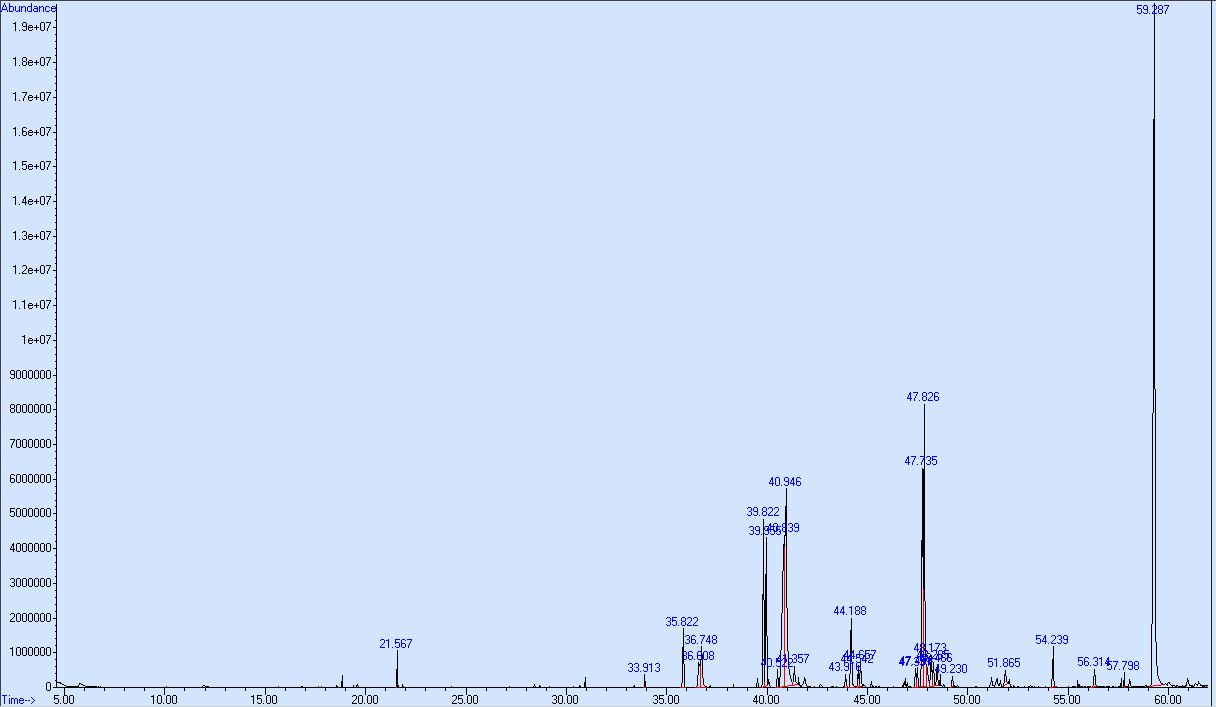
\includegraphics[width=0.8\textwidth]{media/pish/image15}
	\caption*{3-Сурет. Профилтролидың )PROFITROLI\_OBRAZEZ\_2)
	хроматограммасы}
\end{figure}


\begin{multicols}{2}

Зерттеу барсында, тек глютенсіз кондитерлік өнімдерде
(PROFITROLI\_OBRAZEZ\_2) жоғары холестерин мөлшерін 33,93\% құрайтыны
көрсетілген.

Профильтроли құрамындағы өсімдік стеролы (фитостерол) - стигмастерол (Е
499 тізімделген бойынша тағамдық қоспа) мөлшері - 0,79\%, ноқат ұнын
өңдегеннен кейін анықталды, жасуша мембраналарының құрылымы мен
физиологиясын сақтаудың негізгі функциясы бар ең көп таралған заттардың
бірі және LDL холестерин деңгейін төмендетуге қабілетті заттардың да
кездесетіні анықталды. Фитостерол азық-түлік өндірісінде биологиялық
құрамдық мөлшерін арттыруға, сонымен қатар D3 витаминінің прекурсоры
ретінде қарастырылады. Өндірістегі тағамдық қоспалар жартылай
синтетикалық прогестеронд, эстроген әсерлерімен байланысты реттеуші және
тіндерді қалпына келтіру механизмдерінде маңызды физиологиялық рөл
атқаратын, эстрогендер және кортикоидтарқатарына жататын Stigmasterol
қосылысы да зерттеу жұмысы бойынша кездесетіні анықталды. Ол бұршақ
қалдықтардында, тұқымдарында кездеседі. Пастеризацияланған
стигмастеролдарды инактивациялау, тағамдық майларға қарағанды көкеніс
майдарына көбiрек кездеседі.

Зерттеу нәтижелеріне сәйкес, глютенсіз нан өнімдерін дайындау кезінде
микротолқынды өңдеу витаминдердің өзгерістерге ұшыруы (мысалға
профилтроли үлгісінің пайдалана отырып), олар сәйкесінше пайдалы
тағамдық және биологиялық құнды қосылыстарға айналады. Өнімдердің
сапасын бағалау кезінде олардың құрамындағы маңызды полиқанықпаған май
қышқылдарының екі өкілі - линол және линолен қанықпаған жоғары май
қышқылдарының мөлшері үлкен мәнге ие. Екі қышқыл да өсімдік ағзаларының
биосинтезінің өнімдері болып табылады, олар олеин қышқылынан түзіледі.

Зерттеу нәтижелері бойынша, хроматограммалардан көрініп тұрғандай, ноқат
ұнын микротолқынды пешпен өңдеген кезде өңделген ұннан глютенсіз
кондитерлік өнім (профильтроли) сияқты биотехнологиялық қасиеттері
жоғары жаңа өнім алу мүмкін болды.

{\bfseries Қорытынды.} Өңделмеген және өңделген ноқат ұнының және глютенсіз
кондитерлік өнімдердің май қышқылдық құрамын масс-спектрометриялық газ
хроматографиясының ГХ/MС әдісімен анықтау тиімді әдіс болып табылатыны
анықталды.

Зерттелетін объектілер, өңделген ноқат ұны полиқанықпаған май
қышқылдарының көзі үшін перспективалы өнім бола алатынын зерттеу
нәтижесімен дәлелденеді және функциолналдық тағамдарды дайындауда және
аурудың жекелеген түрлерін кешенді емдеу терапиясының бір бөлігінде
пайдалы тағамдық зат ретінде емдеуде қолданылуга болатынын ұсынуға
болады.

Масс-спектрометриялық газ хроматографиясының ГХ/MС әдісімен зерттеу
қорытындысы бойынша жаңадан дайындалған глютенсіз өнімнің (профильтроли)
құрамдық компоненттерінің сандық және сапалық құрамы салыстырмалы
бақылау үлгісімен (өнделмеген ноқат ұнымен) және термиялық өңделген
(негізгі шикізат) ноқат ұндарымен салыстырғанда маңызды және пайдалы
тағамдық диеталық жоғары май қышқылдарының сандық құрамының артқандығы
байқалды:

- олеин қышқылы 12,28 \% -ға дейін;

- линол қышқылы 3,57-ден 28,10\% -ға дейін жоғарлағаны;

- фталь қышқылы 0,62-ден 2,01\%-ға дейін артқандығы,

- пальметин қышқылы 2,16-дан 7,04\%-ға дейін жоғарлағаны;

- стеарин қышқылы 4,35-30,79\% аралығында жоғарлағандығымен дәлелденеді.

Бұршақ тұқымдас дақылдарды микротолқынды пешпен өңдеу (уақыттық қатынас
бойынша) арқылы олардың құрамдық зиянды - улы заттарының сандық
мөлшерінің азаюымен және толық модификациялануы алынған нәтижелер
дәлелденіп және бұл тиімді әдіс екені анықталды.

Осылайша, жүргізілген зерттеулер өнімнің тұтынушылық сапасын және
сақтаудың тұрақтылығын арттыру мақсатында кондитерлік өнімдерді өндіруде
микротолқынды пешті пайдалана отырып, ноқат ұнын «модификациялауды»
қолданудың орындылығын растайды.

Жоғарыда аталған компоненттерді пайдалана отырып, «\emph{пайдалы тағам}»
кондитерлік өнімдерінің жаңа желісін әзірлеу қымбат тұратын импорттық
өнімдерді немесе компоненттерді сатып алуды азайтады.

Бұл зерттеу жұмыстары Қазақстан Республикасы Білім және ғылым
министрлігінің гранттық қаржыландыру AR09561622 «Қазақстанда өсірілетін
бұршақ тұқымдарынан алынған ұнды пайдалана отырып, глютенсіз ұннан
жасалған кондитерлік өнімдерді өндіру технологиясын әзірлеу» тақырыбы
аясында жүргізілді.

Масс-спектрометриялық газ хроматографиясының (ГХ/МС) әдісімен
эсперименттік зерттеу талдауын жасаған Е.Бөкетов атындығы Қарағанды
университетінің «Физика-химиялық зерттеу әдістері» инженерлік бейіндегі
аккредиттелген зертхана орталығына алғыс айтамыз.
\end{multicols}

\begin{center}
	{\bfseries Әдебиеттер}
	\end{center}
	
	\begin{references}

1. Antonella Maggio, Santino Orecchio. Fatty Acid Composition of
Gluten-Free Food (Bakery Products) for Celiac People //Chemistry and
Materials Science. -2018.
DOI:\href{http://dx.doi.org/10.20944/preprints201806.0142.v1}{10.20944/preprints201806.0142.v1}

2. Хорошевская Л. Эффективность использования нута в рационах птицы //
Комбикорма. -2012. -№4. -- С.61-62. URL:
https://kombi-korma.ru/sites/default/files/2/4\_12/04\_2012\_61-62.pdf

3. ГОСТ 8758-76 Межгосударственный стандарт. Нут. Требование при
загатовках и поставках.

4.СанПиН 2.3.2.1078-01. Санитарно-эпидемиологические правила и нормативы
Гигиенические требования безопасности и пищевой ценности пищевых
продуктов

5.Омаралиева А.М., Ботбаева Ж.Т., Агедилова М.Т., Абилова М.,
Жанайдарова А. Влияние СВЧ обработки зернобобовых культур на свойства
безглютеновой муки// Вестник ЕНУ имени Л.Н. Гумилева. Серия
Биологические науки. -2021. -№ 4 (137). --C. 75-83. DOI:
10.32523/2616-7034-2021-137-4-75-83

6. Omaraliyeva A., Botbayeva Zh., Agedilova M.T., Abilova M. Determining
the optimal parameters of ultra-high-frequency treatment of chickpeas
for the production of gluten-free flour // Eastern-European Journal of
Enterprise Technologies. -- 2021. --Vol. 5(11 (113. --P. 51--60. \\DOI:
10.15587/1729-4061.2021.241877

7. Omaraliyeva A., Botbayeva Zh., Agedilova M.T., Abilova M., Nurtayeva
A., Baishugulova Sh.. \\Development of the recipe composition of
gluten-free flour confectionery products based on chickpea flour //
Eastern-European Journal of Enterprise Technologies, Technology and
Equipment of Food \\Production. -- 2022. --Vol. 6 (11) 120. --P. 109 -125.
DOI: 10.15587/1729-4061.2022.269397

8. Etiene V Aguiar, Fernanda G Santos, Ana Carolina L S Centeno, Vanessa
D Capriles Influence of pseudocereals on gluten-free bread quality: A
study integrating dough rheology, bread physical properties and
acceptability//Food Research International. - 2021, Vol. 150. DOI:
10.1016/j.foodres.2021.110762

9. Xu Chen, Xiaowei He, Xiong Fu, Qiang Huang. In vitro digestion and
physicochemical properties of wheat starch/flour modified by
heat-moisture treatment // Journal of Cereal Science. -2015.-Vol 63. -Р.
109-115. DOI: 10.1016/j.jcs.2015.03.003

10. Ainhoa Vicente, Marina Villanueva, Pedro A. Caballero, Athina
Lazaridou, Costas G. Biliaderis, Felicidad Ronda. Flours from
microwave-treated buckwheat grains improve the physical properties and
nutritional quality of gluten-free bread // Food Hydrocolloids. -2024. -
Vol. 149. \\DOI: 10.1016/j.foodhyd.2023.109644

11.Толстогузова Т.Т., Ниязова Д.Р. Разработка рецептуры и технологии
изготовления пряников с использованием муки из нута /Молодой ученый. -
2020. -№ 21 (311). - С. 550-552. \\URL:
https://moluch.ru/archive/311/70338

12. Пащенко Л.П. Разработка технологии хлеба, обогащенного семенами нута
//Журнал Успехи современного естествознания. - 2009. -№ 1. - С. 24-38

13 Намсараева Г.Т., Николаев С.М. Фитотерапия начальных форм хронической
недостаточности мозгового кровообращения. -- Улан-Удэ, 2003. -- 176 с.

14. Громова О.А., Керимкулова Н.В. Нейропротективный эффект
докозагексаеновой и эйкозопентаеновой полиненасыщенных жирных кислот и
перинатальная защита мозга плода (клинико-\\фармакологическая лекция) //
Гинекология. -- 2011. -- № 6. -- С. 30--36.

\end{references}

\begin{center}
{\bfseries References}
\end{center}

\begin{references}

1. Antonella Maggio, Santino Orecchio. Fatty Acid Composition of
Gluten-Free Food (Bakery Products) for Celiac People //Chemistry and
Materials Science. -2018. DOI:10.20944/preprints201806.0142.v1

2. Horoshevskaja L. Jeffektivnost'{}
ispol' zovanija nuta v racionah pticy // Kombikorma.
-2012. -№4. -- S.61-62. URL:
\url{https://kombi-korma.ru/sites/default/files/2/4_12/04_2012_61-62.pdf}
{[}in Russian{]}

3. GOST 8758-76 Mezhgosudarstvennyj standart. Nut. Trebovanie pri
zagatovkah i postavkah. {[}in Russian{]}

4.SanPiN 2.3.2.1078-01. Sanitarno-jepidemiologicheskie pravila i
normativy Gigienicheskie trebovanija bezopasnosti i pishhevoj cennosti
pishhevyh produktov {[}in Russian{]}

5.Omaralieva A.M., Botbaeva Zh.T., Agedilova M.T., Abilova M.,
Zhanajdarova A. Vlijanie SVCh \\obrabotki zernobobovyh
kul' tur na svojstva bezgljutenovoj muki// Vestnik ENU
imeni L.N. Gumileva. Serija Biologicheskie nauki. -2021. -№ 4 (137).
--C. 75-83. DOI: 10.32523/2616-7034-2021-137-4-75-83 {[}in Russian{]}

6. Omaraliyeva A., Botbayeva Zh., Agedilova M.T., Abilova M. Determining
the optimal parameters of ultra-high-frequency treatment of chickpeas
for the production of gluten-free flour // Eastern-European Journal of
Enterprise Technologies. -- 2021. --Vol. 5(11 (113. --P. 51--60. \\DOI:
10.15587/1729-4061.2021.241877

7. Omaraliyeva A., Botbayeva Zh., Agedilova M.T., Abilova M., Nurtayeva
A., Baishugulova Sh.. \\Development of the recipe composition of
gluten-free flour confectionery products based on chickpea flour //
Eastern-European Journal of Enterprise Technologies, Technology and
Equipment of Food\\ Production. -- 2022. --Vol. 6 (11) 120. --P. 109 -125.
DOI: 10.15587/1729-4061.2022.269397

8. Etiene V Aguiar, Fernanda G Santos, Ana Carolina L S Centeno, Vanessa
D Capriles Influence of pseudocereals on gluten-free bread quality: A
study integrating dough rheology, bread physical properties and
acceptability//Food Research International. - 2021, Vol. 150. DOI:
10.1016/j.foodres.2021.110762

9. Xu Chen, Xiaowei He, Xiong Fu, Qiang Huang. In vitro digestion and
physicochemical properties of wheat starch/flour modified by
heat-moisture treatment // Journal of Cereal Science. -2015.-Vol 63. -R.
109-115. DOI: 10.1016/j.jcs.2015.03.003

10. Ainhoa Vicente, Marina Villanueva, Pedro A. Caballero, Athina
Lazaridou, Costas G. Biliaderis, Felicidad Ronda. Flours from
microwave-treated buckwheat grains improve the physical properties and
nutritional quality of gluten-free bread // Food Hydrocolloids. -2024. -
Vol. 149. \\DOI: 10.1016/j.foodhyd.2023.109644

11.Tolstoguzova T.T., Nijazova D.R. Razrabotka receptury i tehnologii
izgotovlenija prjanikov s ispol' zovaniem muki iz nuta
/Molodoj uchenyj. - 2020. -№ 21 (311). - S. 550-552. URL:
\url{https://moluch.ru/archive/311/70338} {[}in Russian{]}

12. Pashhenko L.P. Razrabotka tehnologii hleba, obogashhennogo semenami
nuta //Zhurnal Uspehi \\sovremennogo estestvoznanija. - 2009. -№ 1. - S.
24-38 {[}in Russian{]}

13 Namsaraeva G.T., Nikolaev S.M. Fitoterapija
nachal' nyh form hronicheskoj nedostatochnosti mozgovogo
krovoobrashhenija. -- Ulan-Udje, 2003. -- 176 s. {[}in Russian{]}

14. Gromova O.A., Kerimkulova N.V. Nejroprotektivnyj jeffekt
dokozageksaenovoj i jejkozopentaenovoj polinenasyshhennyh zhirnyh kislot
i perinatal' naja zashhita mozga ploda
(kliniko-farmakologicheskaja lekcija) // Ginekologija. -- 2011. -- № 6.
-- S. 30--36. {[}in Russian{]}

\end{references}

\begin{authorinfo}
\hspace{1em}\emph{{\bfseries Авторлар туралы мәлімет}}

Агедилова М.Т. - химия ғылымдарының кандидаты, Қ.Құлажанов атындағы
Қазақ технология және бизнес университеті, Астана, Қазақстан, «ХБО» АҚ
«Болашақ» түлегі, e-mail: agedilova-2011@mail.ru;

Омаралиева А.М. - техника ғылымдарының кандидаты, Қ.Құлажанов атындағы
Қазақ технология және бизнес университеті, Астана, Қазақстан, e-mail:
\href{mailto:aigul-omar@mail.ru}{\nolinkurl{aigul-omar@mail.ru}};

Ботбаева Ж.Т. - биология ғылымдарының кандидаты, Қ.Құлажанов атындағы
Қазақ технология және бизнес университеті, Астана, Қазақстан, «ХБО» АҚ
«Болашақ» түлегі, e-mail:
\href{mailto:zhanar.b.t@mail.ru}{\nolinkurl{zhanar.b.t@mail.ru}}.

Абилова М.Б. -- магистр технических наук, ассистент, НАО «Казахский
агротехнический университет им.\\ С. Сейфуллина», Астана, Қазақстан,
e-mail: mikentii@inbox.ru

\hspace{1em}\emph{{\bfseries Information about authors}}

Agedilova M.T. - Candidate of Chemical Sciences, JSC Kazakh University
of Technology and Business named after. \\K. Kulazhanov, Graduate of JSC
Center for International Programs Bolashak, e-mail:
\href{mailto:agedilova-2011@mail.ru}{\nolinkurl{agedilova-2011@mail.ru}};

Omaraliyeva A.М. -- Candidate of Technical Sciences, JSC Kazakh
University of Technology and Business named after. \\K. Kulazhanov,
e-mail:
\href{mailto:aigul-omar@mail.ru}{\nolinkurl{aigul-omar@mail.ru}};

Botbaeva Zh.T. - Candidate of Biological Sciences, JSC Kazakh University
of Technology and Business named after. \\K. Kulazhanov, Graduate of JSC
Center for International Programs Bolashak, e-mail: zhanar.b.t@mail.ru.

Abilova M.B. - Master of Technical Sciences, Assistant, S. Seifullin
Kazakh Agro Technical University, Nur-Sultan, Kazakhstan, e-mail:
\href{mailto:mikentii@inbox.ru}{\nolinkurl{mikentii@inbox.ru}}.
\end{authorinfo}
